\subsection{Contexto da pesquisa} \label{subsec:contexto}
\citeonline{mateus} A necessidade de desenvolvimento do planejamento estratégico no mundo corporativo e no dia-a-dia torna a análise de séries temporais e previsões valiosas ferramentas para apoiar o processo de tomada de decisão a curto, médio e longo prazo. Devido às não linearidades, sazonalidade, tendência e ciclicidade nos dados temporais, o desenvolvimento de modelos de previsão eficientes é uma tarefa desafiadora.

No conjunto de dados da SANEPAR, há um volume significativo no consumo de água e, com as interrupções que a cidade tem enfrentado, é necessário analisar os dados para compreender melhor os padrões de interrupção no abastecimento e os picos de consumo ao longo das horas e dias.

Nesta dissertação, será realizada uma revisão sistemática de modelos preditivos para avaliar o melhor modelo que pode ser utilizado e como ele pode ser validado para prever a escassez de água. Essas análises serão feitas utilizando a linguagem de programação \textit{Python}.

A abordagem deste trabalho consiste em explorar o conceito de séries temporais e sua aplicação no campo do aprendizado de máquina. Os dados de séries temporais referem-se a dados coletados e armazenados ao longo do tempo, permitindo que observadores identifiquem anomalias nos dados. A classificação dos dados por ano ou dia é essencial na análise de séries temporais, e se os dados forem atribuídos aleatoriamente, pode ser mais desafiador fazer previsões e tomar decisões com base nos dados coletados.

É importante destacar que a análise de médias pode ser enganosa se não forem excluídos os valores discrepantes, também conhecidos como ``outliers''. Esses valores discrepantes podem levar a resultados extremamente altos ou baixos que não refletem a realidade.
O campo do aprendizado de máquina abrange várias áreas, conforme ilustrado na Figura \ref{fig:paradigma-ml}. Serão explorados os diferentes componentes do aprendizado de máquina e como eles podem ser aplicados em diversos contextos.
 
\begin{figure}[!hb]
	\centering
	\caption{Paradigma de aprendizado de máquina}
	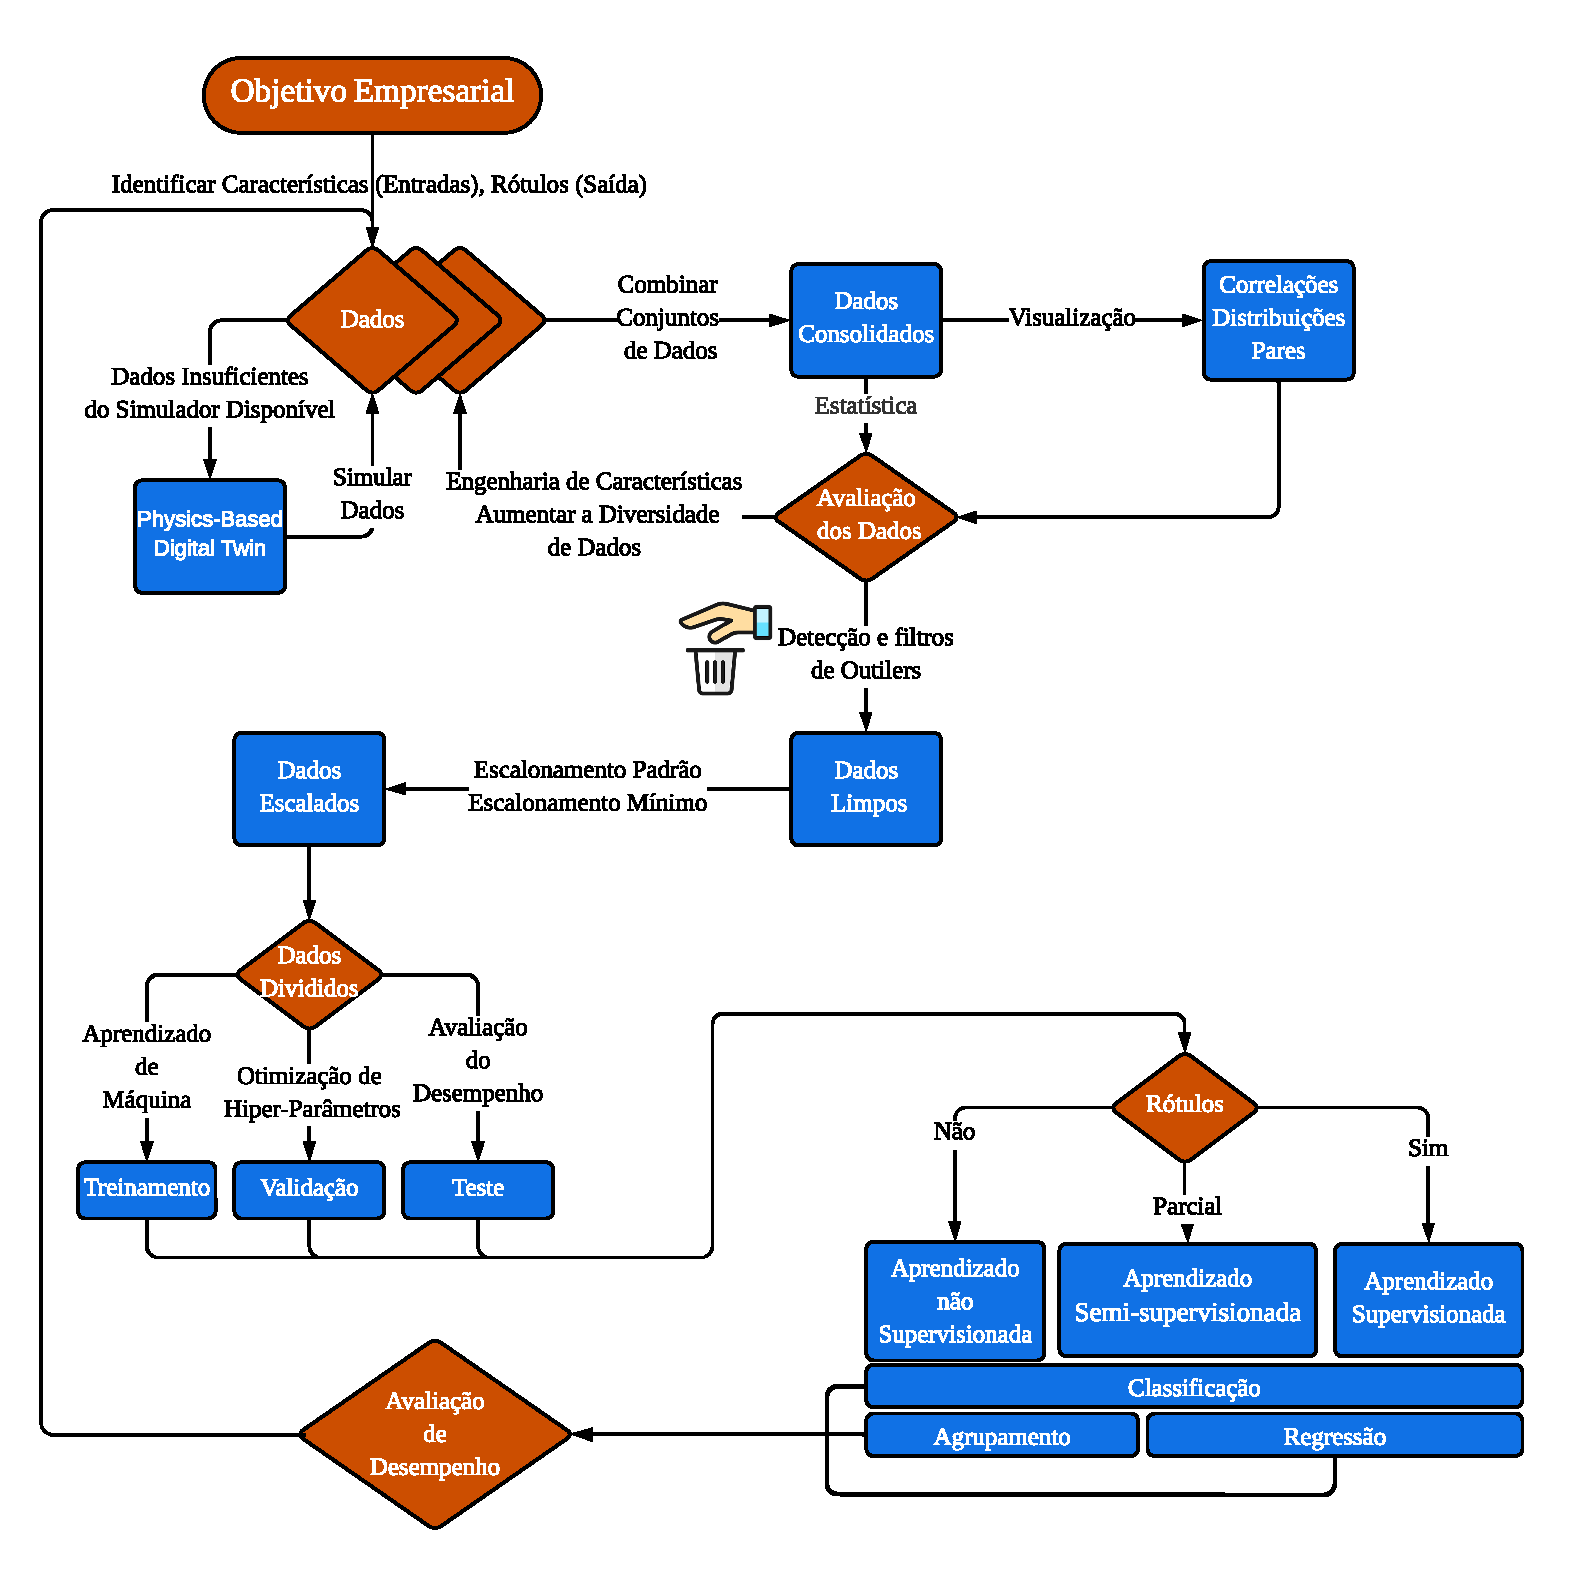
\includegraphics[width=1\linewidth]{Introducao/Figuras/paradigma-ml}
	
	\fonte{Elaboração própria}
	\label{fig:paradigma-ml}
\end{figure}
  
      
\subsubsection{Motiva\c c\~ao da pesquisa} \label{subsubsec:motivacao}
 
 
 	A motivação desta pesquisa é baseada na situação enfrentada por Curitiba e região metropolitana, conforme apontado por \citeonline{vasconcelos_2020}. A região passou por um rodízio de abastecimento de água, com períodos de 36 horas com água seguidos por 36 horas sem abastecimento. A média geral dos reservatórios na região estava em torno de $27,96\%$ de sua capacidade. Além disso, a quantidade de chuva nos anos anteriores, de $2020$, foi de $1.704 \ mm$, superando a média anual de precipitação de $1.490 \ mm$.
 	
 	Diante dessa situação, a pesquisa tem como abordagem principal a escassez de água, que pode ser associada a condições de seca. A partir dos dados coletados pela SANEPAR, é possível realizar uma análise mais detalhada, com o objetivo de prever e evitar a ocorrência de escassez de água, que foi registrada como uma anomalia em $2020$. Com o retorno das chuvas, houve um aumento nos níveis dos reservatórios, o que torna essencial a análise e previsão dos dados para um melhor planejamento e gerenciamento do abastecimento de água na região.
    
     
    